\documentclass[../../main/thesis_msc.tex]{subfiles}



\begin{document}

	\chapter{Type-Ia Supernovae from non-accreting progenitors}
	
	John Antoniadis, \textbf{Savvas Chanlaridis}, G\"otz Gr\"afener, and Norbert Langer (2019)[in preparation]
	\newline
	
	\begin{center}
	\textbf{\large Abstract}
	\end{center}
	
	Type Ia supernovae (\ias) are  manifestations of helium-deficient stars disrupting in a 
	thermonuclear runaway. While explosions of carbon-oxygen white dwarfs are 
	thought to account for the majority of events, part of the observed diversity 
	may be due to varied progenitor channels. We demonstrate that 
	helium stars with masses between 1.8 and 2.5\msun\ may evolve 
	into highly degenerate, near-Chandrasekhar mass cores with 
	helium-deficient envelopes, that subsequently  ignite carbon and oxygen explosively at densities $\sim10^{9.26-9.77}$ \,gr\,cm$^{-3}$. 			This happens either due to compression from 
	shell burning (when the core has a hybrid CO/NeO composition), 
	or following ignition of residual carbon triggered by  
	exothermic electron captures on \iso{Mg}{24} (for a 
	NeOMg-dominated  composition). We argue that the resulting 
	thermonuclear runaways are likely to prevent core collapse, 
	leading to the complete disruption of the star in a \ia 
	explosion with a kinetic energy of $\sim 10^{51}$\,erg. 
	The frequency of progenitor systems would suffice to account  
	for a large fraction of \ias in star-forming  galaxies.
	
	\section{Introduction} \label{sec:intro}

 Despite their central role in Astrophysics and Cosmology, 
 the origin and physics of Type Ia supernovae (\ias)
remain uncertain  \citep[][]{Maoz:2013hna}. 
Typical \ia  luminosities ($\sim 10^{43}$\ergs) and ejecta velocities  
($ \sim 10^{4}$\kms), require \iso{Ni}{56}  
masses and kinetic energies of order 
$\sim 0.6$\msun\ and $\sim 10^{51}$\erg\ respectively. 
 These properties suggest that \ias are most likely 
 stars that disrupt in  thermonuclear explosions, 
 rather than core-collapse events. 
 Carbon/oxygen white dwarfs (CO WDs) 
 approaching the Chandrasekhar-mass limit (\mch)
 are the most promising progenitor systems, as they can 
 produce explosions broadly consistent with observations
 \citep{Nomoto:1982zz,Churazov:2014bga}. %Wang:2012za,
 
Conventional stellar evolution channels, produce stable CO WDs with masses below $\sim 1.0$\msun. 
Consequently, matter accretion onto the WD is required to trigger an 
explosion, either via stable  transfer from a 
donor star (single-degenerate channels; SD), or in a 
merger event (double-degenerate channels; DD).  
Thus far, all of the proposed SD or DD variants    
encounter substantial difficulties in providing 
a self-consistent model for \ias \citep{Livio:2018rue}. 
For instance, SD channels require considerable fine-tuning
of the mass accretion rate for
the WD to grow in mass. In addition, the interaction between  
the SN blast and the donor star or the circumbinary material, is expected to produce  signatures which 
are rarely or never seen, e.g. some contribution to the SN  luminosity 
at early times \citep{Kasen:2009si}, radio synchrotron emission 
\citep{Harris:2016hfr}, and H$\alpha$ lines due to unburned hydrogen. 
DD mergers on the other hand may produce a variety of outcomes, 
ranging from prompt 
explosions to long-lived remnants, or the delayed formation of a neutron star \citep{Livio:2018rue}. In addition, their overall contribution to the observed \ia rate may be too low \citep{vanKerkwijk:2010he,claeys2014a,Sato:2015spa}. %Maoz:2013hna


Over the past 50 years, systematic studies of \ia explosions have revealed a large
diversity in their properties \citep{Taubenberger:2017hoo}. 
Examples of extreme outliers include luminous 
\citep[e.g. SN\,1991T;][]{filippenko1992} and ultra-luminous  
\citep[e.g. SNLS-03D3bb;][]{Howell:2006vn} SNe, SN\,1991bg-like transients which
are faint and rapidly evolving \citep{ruiz-lapuente1993},  
and SN\,2012ca-like events, dubbed SNe Ia-CSM, in which 
there is evidence for interaction with a dense circum-stellar 
medium \citep{Bochenek:2017vok}. 
Even among ``normal'' \ias there is appreciable
scatter in rise times, maximum luminosities, ejecta velocities and spectral evolution   
\citep[][]{Livio:2018rue}. 
Finally, there seems to be a correlation with environment, 
as active  galaxies typically  host more,  and brighter \ias \citep{Maoz:2013hna}. 


While part of this diversity can be understood within the framework of SD and DD 
families, there may exist additional 
evolutionary pathways leading to \ias. 
Here, we explore an alternative channel in which a thermonuclear runaway leading to a \ia can be initiated during the late evolution of a degenerate core of neon-oxygen 
(NeO) or carbon-neon-oxygen (CNeO) composition that approaches  \mch. 
Such progenitors are generally thought to produce massive WDs or     
electron capture supernovae (ECSN)  
\citep[e.g.,][]{nomoto1991,gutierrez1996,Takahashi:2013ena}. %However, recent 
%hydrodynamical simulations indicate that if explosive oxygen %at relatively low densities, the star most likely disrupts instead of imploding 
%\citep{Jones:2018ule}. 
%In addition, the presence of residual unburned carbon has been 
%found to have an important influence on the energetics at  late evolutionary stages \citep{Willcox:2016yyp,Schwab:2018cnb}. 
Here however, we show that near-\mch\ \one cores originating from intermediate mass helium stars ($\sim 1.8-2.5$\msun) ---a common product of binary interactions--- can ignite their residual carbon and oxygen explosively at  
densities $\lesssim 10^{9.77}$\,gr\,cm$^{-3}$, 
before the onset of {\rm $^{20}$Ne(e$^-$,$\nu_e$)$^{20}$Fe} 
electron capture reactions (Section\,\ref{sec:2}). 
In addition, the envelope is promptly lost via winds or due to binary interactions, leaving behind a helium-free structure.  
We demonstrate that the combination of 
final composition and available energy, 
would yield explosions with luminosities and ejecta velocities 
consistent with classical \ias (Section\,\ref{sec:3}). 
 This mechanism  does not require accretion from the binary companion and 
 therefore may contribute significantly to the \ia  rate in young stellar populations (Section\,\ref{sec:4}). 
 
% The text is organized as follows. In Section\,\ref{sec:2} we briefly review the evolution of  super-AGB stars and present our results for two representative helium-star progenitor models, evaluated using the 
%\textit{Modules for Experiments in Stellar Astrophysics}  
%\citep[\mesa;][]{Paxton:2010ji,Paxton:2013pj,Paxton:2015jva,Paxton:2017eie}. 
%In Sectios\,\ref{sec:3} and \ref{sec:4},  we provide  zeroth-order estimates for the energetics and  \ia rates respectively. Finally, in 
%Section\,\ref{sec:5} we conclude with a broader discussion on some possible implications and directions for future research. 


\section{\one cores: formation and evolution}\label{sec:2}
Highy degenerate stellar cores of neon-oxygen composition form inside stars with ZAMS masses  
between  7 and 11\msun\ \citep{Farmer:2015afs,Woosley:2019sdf}. 
After core helium burning, such stars enter a super-asymptotic giant branch 
(SAGB) phase, characterized by a dense CO  
core and an  extended hydrogen envelope.  
As the core becomes increasingly more degenerate, it cools substantially 
due thermal neutrino emission. An important consequence is that the critical 
temperature for \iso{C}{12} ignition is first attained off-center, creating a 
convectively bound  flame that propagates inwards \citep{siess2006}. 
%\deleted{converting the chemical composition to
%to primarily neon, oxygen, sodium and magnesium.}  

Carbon burning in SAGB stars is affected by complex mixing processes 
due to a combination of inverse composition gradients, overshooting, 
semi-convection and rotation. The penetration of 
NeONaMg ashes into unburned regions, may impact significantly the propagation of
the burning front. Mixing generally reduces the thermonuclear reaction rate, leaving 
behind substantial amounts of residual carbon. In extreme cases, the flame can be 
quenched completely, resulting in a hybrid structure,  with a CO core, 
surrounded by a NeO mantle \citep{Denissenkov:2013qaa}. 

The subsequent evolution and final fate of the star depend  critical on the competition 
between neutrino cooling due to the presence of \iso{Na}{23}\iso{Ne}{23} and 
\iso{Mg}{25}\iso{Na}{25} Urca pairs, and compressional heating due to accretion from the helium burning shell \citep{Schwab:2017epw}. 
SAGB stars are subject to significant dredge-up  and 
thermally unstable shell burning. 
These effects may impact substantially the ability of the core to grown in mass fast enough. 

However, thermal pulses and dredge-up episodes do not 
occur when the hydrogen envelope 
is lost, e.g. due to a common envelope (CE) event in a binary system \citep{Woosley:2019sdf}.  
In such a case, helium shell burning is stable, allowing  
the core to approach the Chandrasekhar mass limit. 
In what follows, we build detailed numerical models to 
investigate the combined effects 
of residual unburned \iso{C}{12}, Urca cooling and constant mass accretion from shell 
burning, in the late evolution of \one cores that originate from helium stars. 

\subsection{Numerical Calculations: Input Physics}\label{sec:2.1}
We use \mesa version 10386 to follow the evolution of two helium-star models, \textsc{m1} and \textsc{m2}, with  masses of  2.4 and 1.8\msun\ respectively. 
The initial models have uniform compositions with $Y=0.98$ and $Z=0.02$ \citep[solar abundances are taken from ][]{grevesse1998}. We employ a nuclear network that considers 43  isotopes, from \iso{H}{1} to \iso{Ni}{58}. Reaction rates are based on the \texttt{JINA reaclib v2.0} compilation \citep{cyburt2010}. Electron screening factors and cooling rates from thermal neutrinos are evaluated as in \cite{Farmer:2015afs}, and references therein. 
Weak interaction rates are taken from \cite{Suzuki:2015iry}. 
Wind mass loss rates are calculated using \mesa's \texttt{Dutch} compilation   \citep{Paxton:2013pj}. 

Our baseline convection model considers standard, thermohaline and semiconvectional mixing. Convective stability is 
evaluated using the Ledoux criterion. By default, \mesa uses  standard mixing-length theory  \citep[MTL;][]{cox1968} for convective mixing and energy transport. However, following carbon burning, both our models develop 
dynamically-unstable super-Eddington envelopes, causing numerical 
difficulties. For this reason, we decided to employ the ``enhanced'' MLT 
option available in \mesa \citep{Paxton:2013pj}, which artificially reduces 
the super-adiabatic gradient leading to  an enhanced convective energy 
transport efficiency.  This  allows us to follow the evolution of the core 
after carbon burning without interruptions. We further discuss this choice and its impact on the envelope evolution and the final mass in Section\,\ref{sec:5}. 
The MLT mixing length parameter is set to $a_{\rm MLT}=2.0$ for both models. For thermohaline and semi-convection we employ the \cite{kippenhahn1980} and \cite{langer1983} treatments respectively. 
In addition to the baseline mixing parameters, in \textsc{m2}, we also 
consider the effects of overshooting, adopting an efficiency of $f_{\rm ov}=0.014$ across all convective boundaries, including the base of the 
carbon-burning flame. While mixing at this interface may not occur in reality, 
we use this as a means to  quench the flame before reaching the center.  
Other mixing processes such as rotation and thermohaline can lead to the 
same outcome for similar initial helium core masses \citep{Farmer:2015afs}.
The \mesa inlists are publicly available\footnote{\url{http://cococubed.asu.edu/mesa_market/inlists.html}}. 
A more extended grid which explores a broad range of initial masses, 
metallicities and overshooting parameters will be presented in an 
accompanying paper \citep{chanlaridis2019}.       



\subsection{Simulation results}
Figure\,\ref{fig:1} shows Kippenhahn diagrams for 
 \textsc{m1} and \textsc{m2}, focusing on the evolution after central helium depletion.
\begin{figure*}[htb!]
  \centering $
  \begin{array}{cc}
  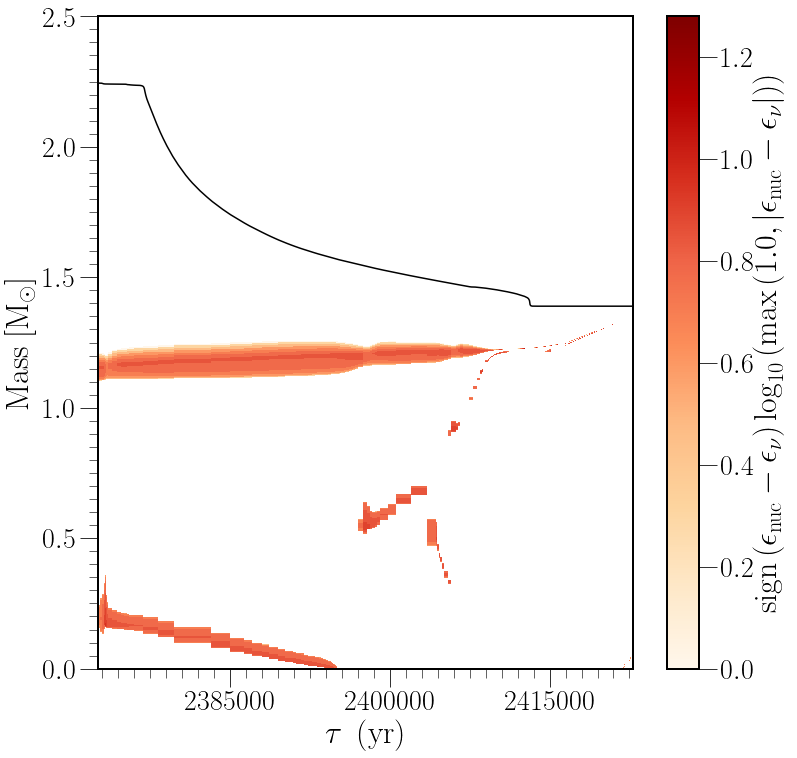
\includegraphics[width=0.5\textwidth]{../figures/chapter3/Kip_m1.png} &
  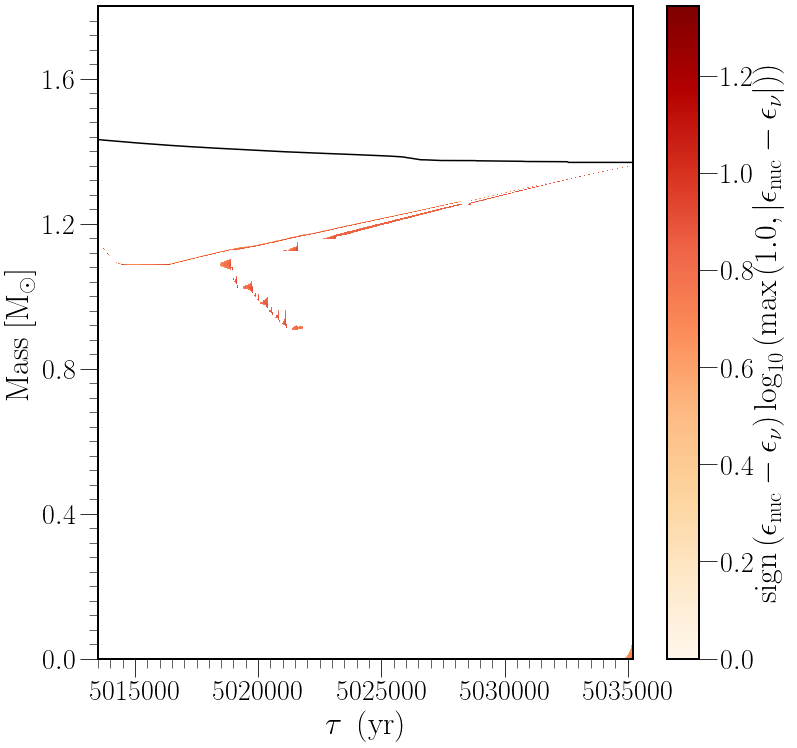
\includegraphics[width=0.5\textwidth]{../figures/chapter3/Kip_m2.png} \\
  \end{array}$
  \caption{Kippenhahn diagrams following the evolution of \textsc{m1} (left) and \textsc{m2} after core helium depletion. Colored areas indicate regions in which nuclear burning occurs, i.e. locations for which the nuclear energy $\epsilon_{\rm nuc}$ exceeds energy losses due to neutrion emission, $\epsilon_\nu$.}
  \label{fig:1}
\end{figure*}
\textsc{m1} first ignites carbon at mass coordinate $\sim 0.3\msun$, when the total mass  is $ 2.25\msun$ and the CO core has a mass of $\sim 1.15\msun$.  
The initial flame is followed by secondary flashes which propagate in both 
directions. Some of these episodes seem to occur only after a small critical 
mass of carbon has been accumulated below the burning shell. The entire carbon-burning phase lasts for about 
40,000\,yr. During most of this time, the star is a red giant with a low-density convective envelope  
($R\simeq 125\rsun$, $\logteff\simeq 3.75$, $\logl\simeq 
4.3$), and loses mass at a rate of  
$\mdot\simeq10^{-6}\mdotsun$, in good agreement with 
recent \textsc{kepler} models \citep{Woosley:2019sdf}. 

As the core contracts and its surface gravity increases, the surrounding burning shells become progressively thinner. The envelope responds by expanding  and the stellar structure resembles closely that of an SAGB star.
The last $\sim 5,000$\,yr of the evolution are characterized by rigorous burning in two neighbouring shells which eventually merge, resulting in a \iso{Ne}{20} flash. In this phase the star reaches extremely high luminosities up to $\log{L/L_\odot = 6.25}$ resulting in a strong stellar wind that lasts for $\sim$1000\,yr and eventually removes the He-rich envelope.

The evolution of the envelope during the final stages 
depends critically on the energy transport mechanism above Eddington lumonisities. With the enhanced MLT option 
employed in our calculations, \textsc{m1} briefly 
becomes a yellow supergiant as the envelope  expands to $R\simeq 900\rsun$ while remaining dynamically stable.
The strong wind of $\mdot\simeq10^{-3.8}\mdotsun$ in this phase is in the same range as theoretically expected maximum values for super-Eddington winds \citep[][]{Owocki:2004zz,Smith2006}.
%
%\deleted{This also results in a sustained wind of $\mdot\simeq10^{-3.8}\mdotsun$, lasting for $\sim$1000\,yr. This brief mass-loss phase is perhaps not too unrealistic, as partial recombination of the carbon-rich  material would increase the porosity, leading to continuum-driven mass loss of similar magnitude \citep[e.g.][]{Owocki:2004zz}.}

Conversely, using standard MLT, the envelope becomes dynamically unstable and our calculations encounter numerical difficulties just as the star leaves its Hayashi track, when the core has a mass of 1.32\msun.
By extrapolating the core-growth rate, the star would likely still reach the  Chandrasekhar limit \citep[see ][for a similar conclusion]{Woosley:2019sdf}. 
More realistically, binary interactions would easily remove the envelope at this stage, as its binding energy corresponds to only a minuscule fraction of the orbital energy reservoir. 

Interestingly, the combination of enhanced mass loss and vigorous burning, leads to the complete depletion of helium in the envelope. 
Following the thermal flash, the small residual envelope contracts and the wind ceases completely for the last $\sim$5,000\,yr (Figure\,\ref{fig:1}). Our model stops when the star has a mass of 1.39\msun~ (see Sec.\,\ref{sec:runway}).  

The surface evolution of \textsc{m2} is similar (Figure\,\ref{fig:1}). Here, 
the star expands twice, first for $\sim$5,000\,yr, and then very briefly for some 
$\sim$500\,yr, reaching a maximum size of $300\rsun$. The mass-loss rate however, always remains 
below $10^{-6}\mdotsun$. In \textsc{m2}, carbon ignites near mass coordinate $1\msun$, 
just as the star begins to develop an SAGB structure. The flame is quenched after only 
$0.1\msun$ of material has been converted to NeO, leaving behind a hybrid CO/NeO structure. Independently of whether this composition profile survives \citep{brooks2017}, the amount of residual  carbon is substantial. This model has a final mass of 1.37\msun. 

To summarise, during the final evolutionary stages, both models are helium 
depleted and nearing \mch. The ability of the core 
to grow in mass depends somewhat on the uncertain mass-loss rate during the final burning phases. If the envelope 
is lost too early during the SAGB phase (which does not seem to be the case), then the two stars would 
leave behind white dwarfs with masses $\le 1.38\msun$, and ONe and CO/ONe composition respectively. 

Conversely, if the envelope is retained for long enough, then the central density increases sufficiently to trigger either electron captures on \iso{Mg}{24} or central carbon ignition. 
In the following section we examine the evolution of the core during this phase. 




\subsection{Late evolution and thermonuclear runaway}\label{sec:runway}
Figure\,\ref{fig:2} gives an overview of the central density and temperature evolution for models  \textsc{m1} and \textsc{m2}. %\deleted{(in blue and orange respectively)}.

Following the main carbon-burning episode, both stars continue to contract, while cooling  due to neutrino  emission. As shell 
burning intensifies, compressional heating eventually balances 
off neutrino losses, at $\logrhoc \simeq 8.3$ and 8.0 for \textsc{m1} and \textsc{m2} respectively. The subsequent evolution depends on the composition. 
\begin{figure*}[htb!]
\begin{center}
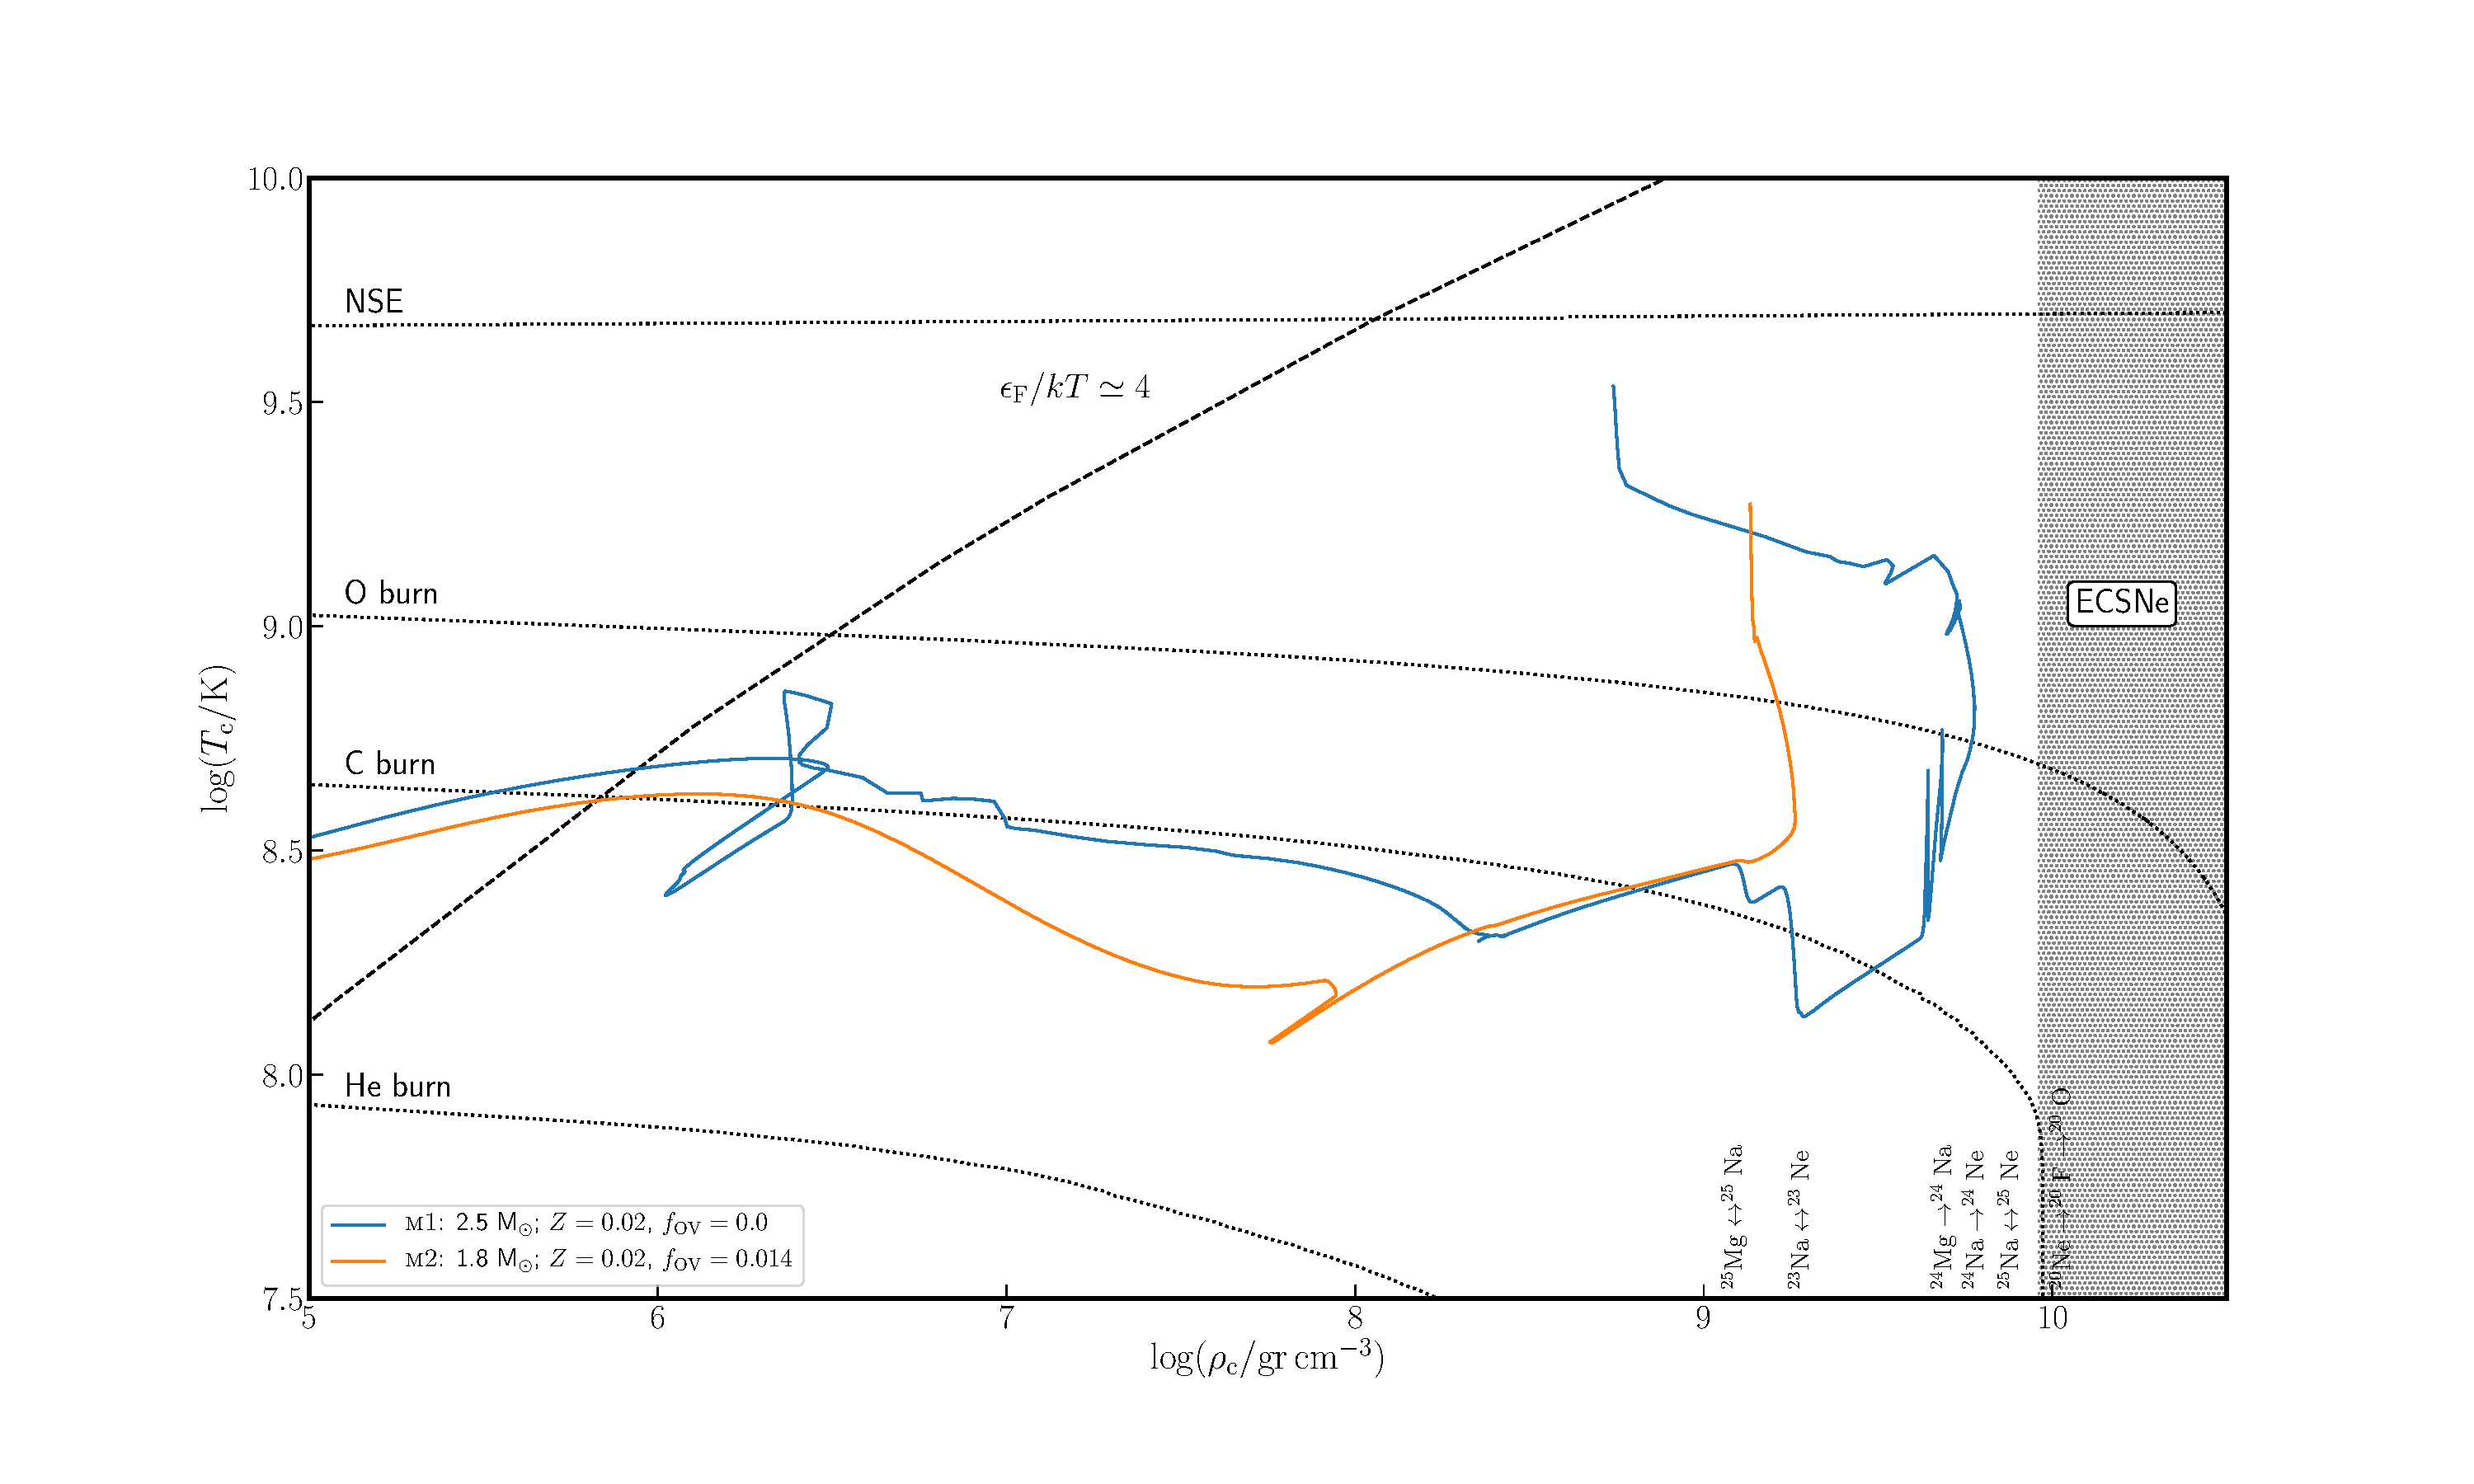
\includegraphics[width=1.0\textwidth]{../figures/chapter3/Rhoc_vs_Tc.pdf}
\caption{Evolution of the core density and temperature for \textsc{m1} and \textsc{m2}. The dashed line shows the approximate boundary for electron degeneracy. Burning thresholds for a 100\% abundace of the corresponding species are indicated with dotted lines. The NSE threshold assumes an equilibrium timescale of 1\,s.}
\label{fig:2}
\end{center}
\end{figure*}
For \textsc{m1}, the degenerate core is composed 
mostly of neon and oxygen. The most abundant isotopes have  $\abun{O}{16}\simeq 0.43$;  $\abun{Ne}{20}\simeq 0.42$; $\abun{Mg}{24}\simeq0.1$;  $\abun{C}{12}\simeq 0.011$; $\abun{Na}{23}\simeq 0.037$; $\abun{Mg}{25}\simeq 0.001$. Between $\logrhoc=9.05$ and 9.25, the temperature drops to $\logtc\simeq 8.2$ due to \iso{Mg}{25}\iso{Na}{25} and \iso{Na}{23}\iso{Na}{23} direct Urca reactions. At higher densities, neutrino cooling ceases completely, and the temperature rises again, along the adiabatic curve shown in Figure\,\ref{fig:2}.  

When $\logrhoc=9.65$, exothermic electron captures on \iso{Mg}{24} and 
\iso{Na}{24} start occurring at a substantial rate, raising the temperature 
adequately to ignite carbon. In turn, this triggers oxygen burning and a thermonuclear runaway at  $\logrhoc= 9.77$. This ignition density is much lower than the   $\logrhoc\ge 9.97$ typically expected for oxygen deflagrations  in pure NeO cores \citep{Jones:2018ule}. As a consequence, severe deleptonization due to \iso{Ne}{20} electron captures are avoided. 

\textsc{m2} is composed mostly of carbon and oxygen, with $\abun{C}{12}=0.38$ and $\abun{O}{16}=0.60$ respectively. 
 Here, \iso{Na}{23} is not abundant enough to cause  substantial cooling. Consequently, carbon, which is significantly more abundant compared to \textsc{m1}, ignites at $\logrhoc=9.26$. 
 
The evolution following central oxygen ignition is not adequately modeled in our 1D simulations. 
 \textsc{m2} will most likely disrupt in a \ia, as the composition and
 ignition conditions resemble closely those found in standard CO WD 
 progenitors \citep{Nomoto:1982zz}. While the fate of \textsc{m1} is less 
 certain, a thermonuclear explosion is also the most likely outcome: 
 firstly, the available nuclear energy is sufficient to unbind the star (see 
 below). Secondly, the ignition density is not too much higher than the $\logrhoc\simeq9.3-9.7$ expected for CO WD progenitors. Hence, the 
 deflagration ashes will likely be buoyant, leading to expansion, which will 
 in turn limit the deleptonization rate. This hypothesis is strongly supported
 by 3D hydrodynamic  simulations of ECSN deflagrations by \cite{Jones:2018ule}: their least compact progenitor ingites at $\logrhoc=9.90$ but still manages to eject  $\sim 1\msun$ of material. 
 Similarly,  \cite{marquardt2015} simulate ONe WD detonations at lower 
 densities and demonstrate that the explosion is practically identical to a 
 typical \ia. 
 Interestingly in our 1D simulations, both models experience significant expansion. This is most likely the result of (over-)efficient convection, which also homogenizes the inner $\sim 1\msun$ of the core. 
 
 
 
 

\subsection{Energetics and nucleosynthesis}\label{sec:3}
Figure\,\ref{fig:nuc} shows the density profiles of \textsc{m1} and \textsc{m2} at maximum compactness, and at the end of our simulations. At the onset of oxygen ignition, \textsc{m1} and \textsc{m2} have internal energies (gravitational+thermal) of $-5.76$ and $-5.16$\,erg, and average electron fractions of $\ye= 0.496$ and  0.499 for \textsc{m1} and \textsc{m2} respectively. If these progenitors were to produce an \ia of  typical composition of $\sim 0.7\msun$ of nickel and iron and 0.6\msun of Si-group elements, the corresponding kinetic energies would be $E_{\rm \textsc{m1}}\simeq 0.83$ and $E_{\rm \textsc{m2}}\simeq 1.17\times10^{51}$\,erg, consistent with observations. 
Obviously, the nucleosynthesis yields depend on the actual
\ye\ and density profiles during explosive burning. If 
\textsc{m1} achieves nuclear statistical equilibrium (NSE)
without significant expansion and deleptonization, then it
would produce mostly stable iron-peak elements and $\sim 0.3\msun$ of \iso{Ni}{56}, resulting in a sub-luminous 
explosion. On the other hand, if NSE is achieved after an 
initial deflagration (Figure\,\ref{fig:nuc}), then up to 
1\msun\ of \iso{Ni}{56} can be produced, with only moderate
amounts of iron. Similarly, \textsc{m2} could produce up 
to 1.3\msun\ of iron elements if it doesn't expand any 
further. 

\begin{figure}
\begin{center}
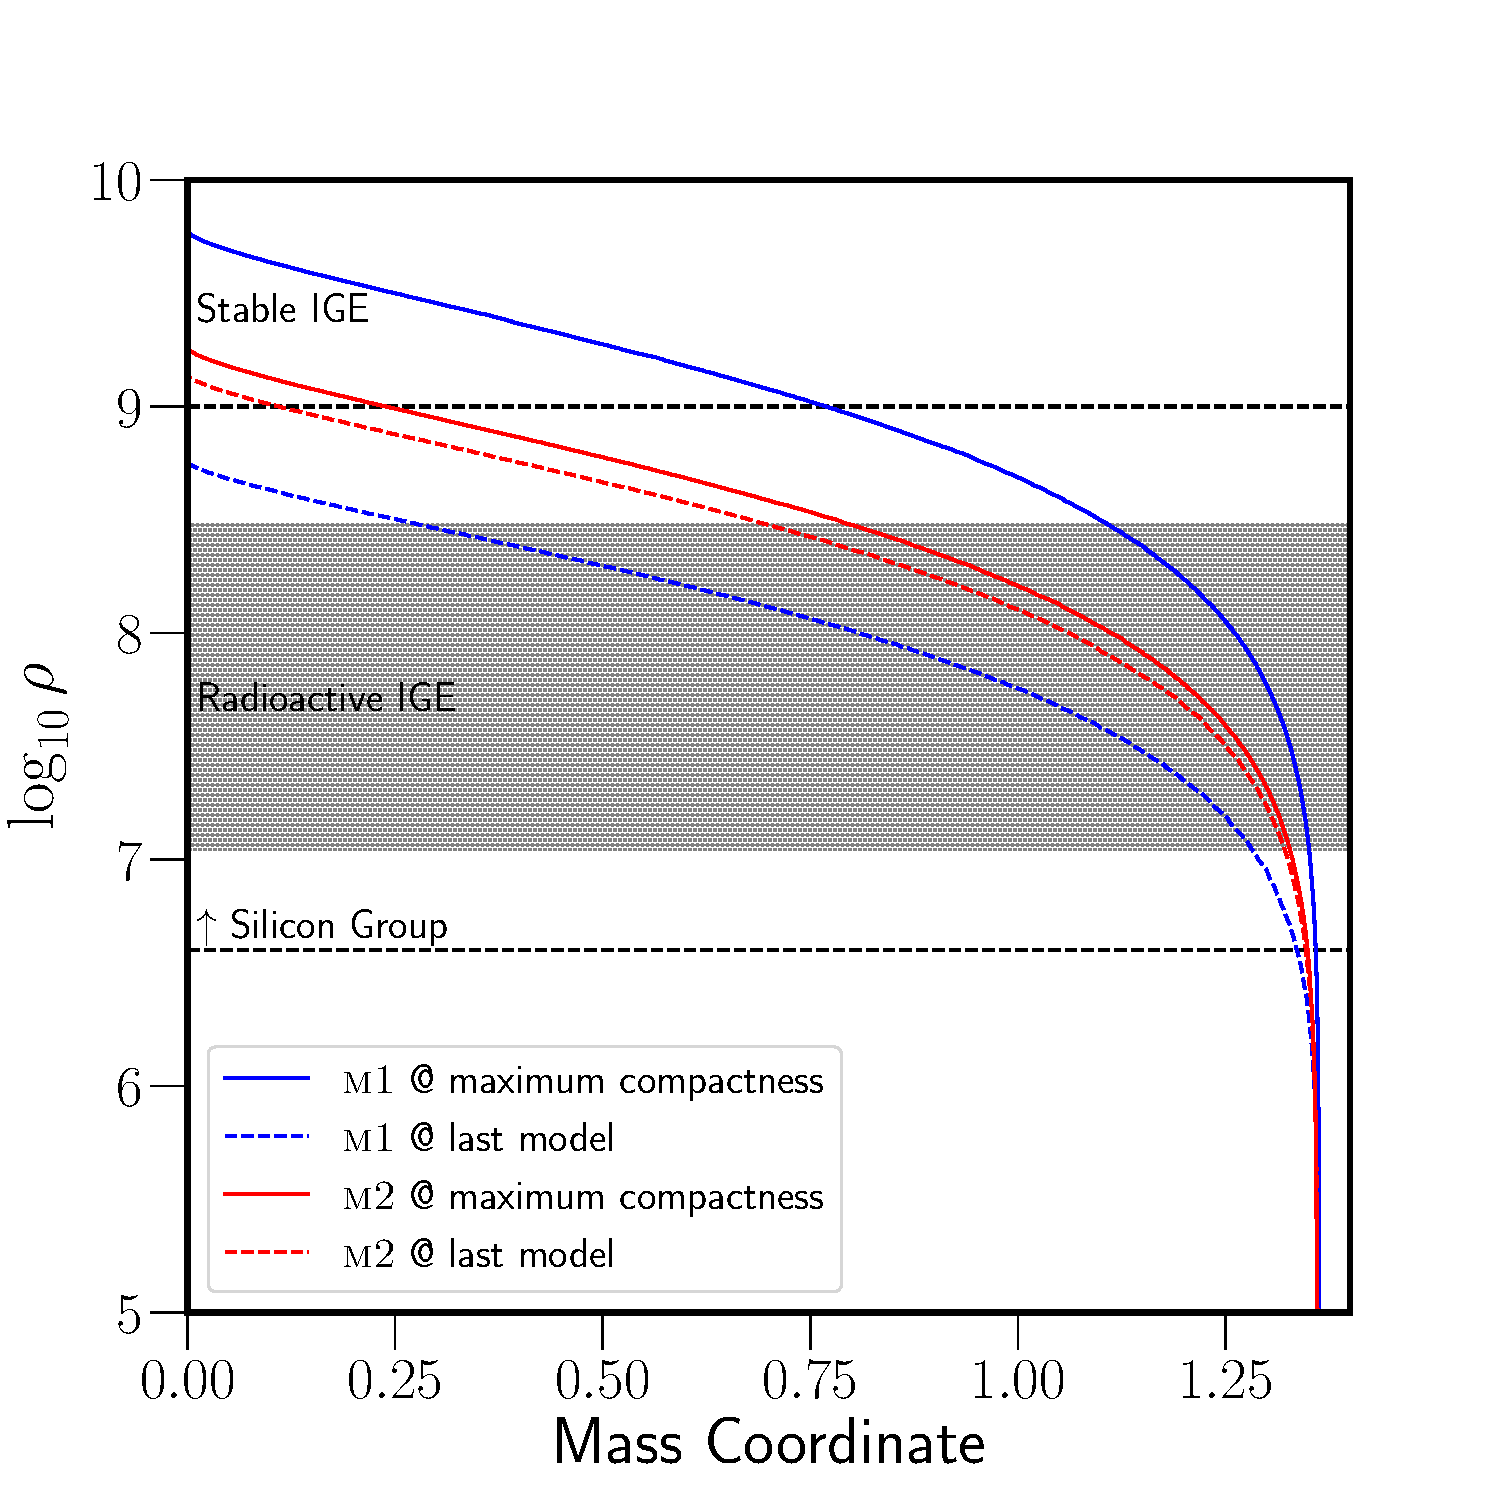
\includegraphics[width=0.5\textwidth]{../figures/chapter3/composition.pdf}
\caption{Density profiles at maximum compactness (solid lines) and at the end of our \mesa calculations (dashed lines). Regions indicating approximate burning regimes as in \cite{Seitenzahl2017}.}
\label{fig:nuc}
\end{center}
\end{figure}


\section{Expected rates and delay times}\label{sec:4}
A useful proxy for the potential \one/\ia connection would be a comparison between 
the  Hubble-integrated number of \ias, n$_{\rm \ia}$, and the expected frequency  of stripped  near-Chandrasekhar mass \one cores, $n_\star$. Here, we provide an
order-of-magnitude estimate to demonstrate that the two may indeed be similar. 

To first order, $n_\star$ would be some fraction of the initial star-forming mass that will end up creating    \one cores. Since the  envelope needs to be removed before the onset of core helium burning, these stars would also need to be members of close  binary systems, thus:  
\begin{equation}
n_{\star} \simeq  f_{\rm bin} \times f_{\rm int} \times  n_{\rm \one}.
\end{equation}
Here, $f_{\rm bin}\simeq 0.7$ \citep{Sana:2012px} is the stellar binary fraction,   $n_{\rm \one}$ is the total 
number of stars able to form \one cores, and $f_{\rm int}\leq 1$ is an efficiency factor to account for the impact of binary interactions (see below).
\begin{figure*}[htb!]
\begin{center}
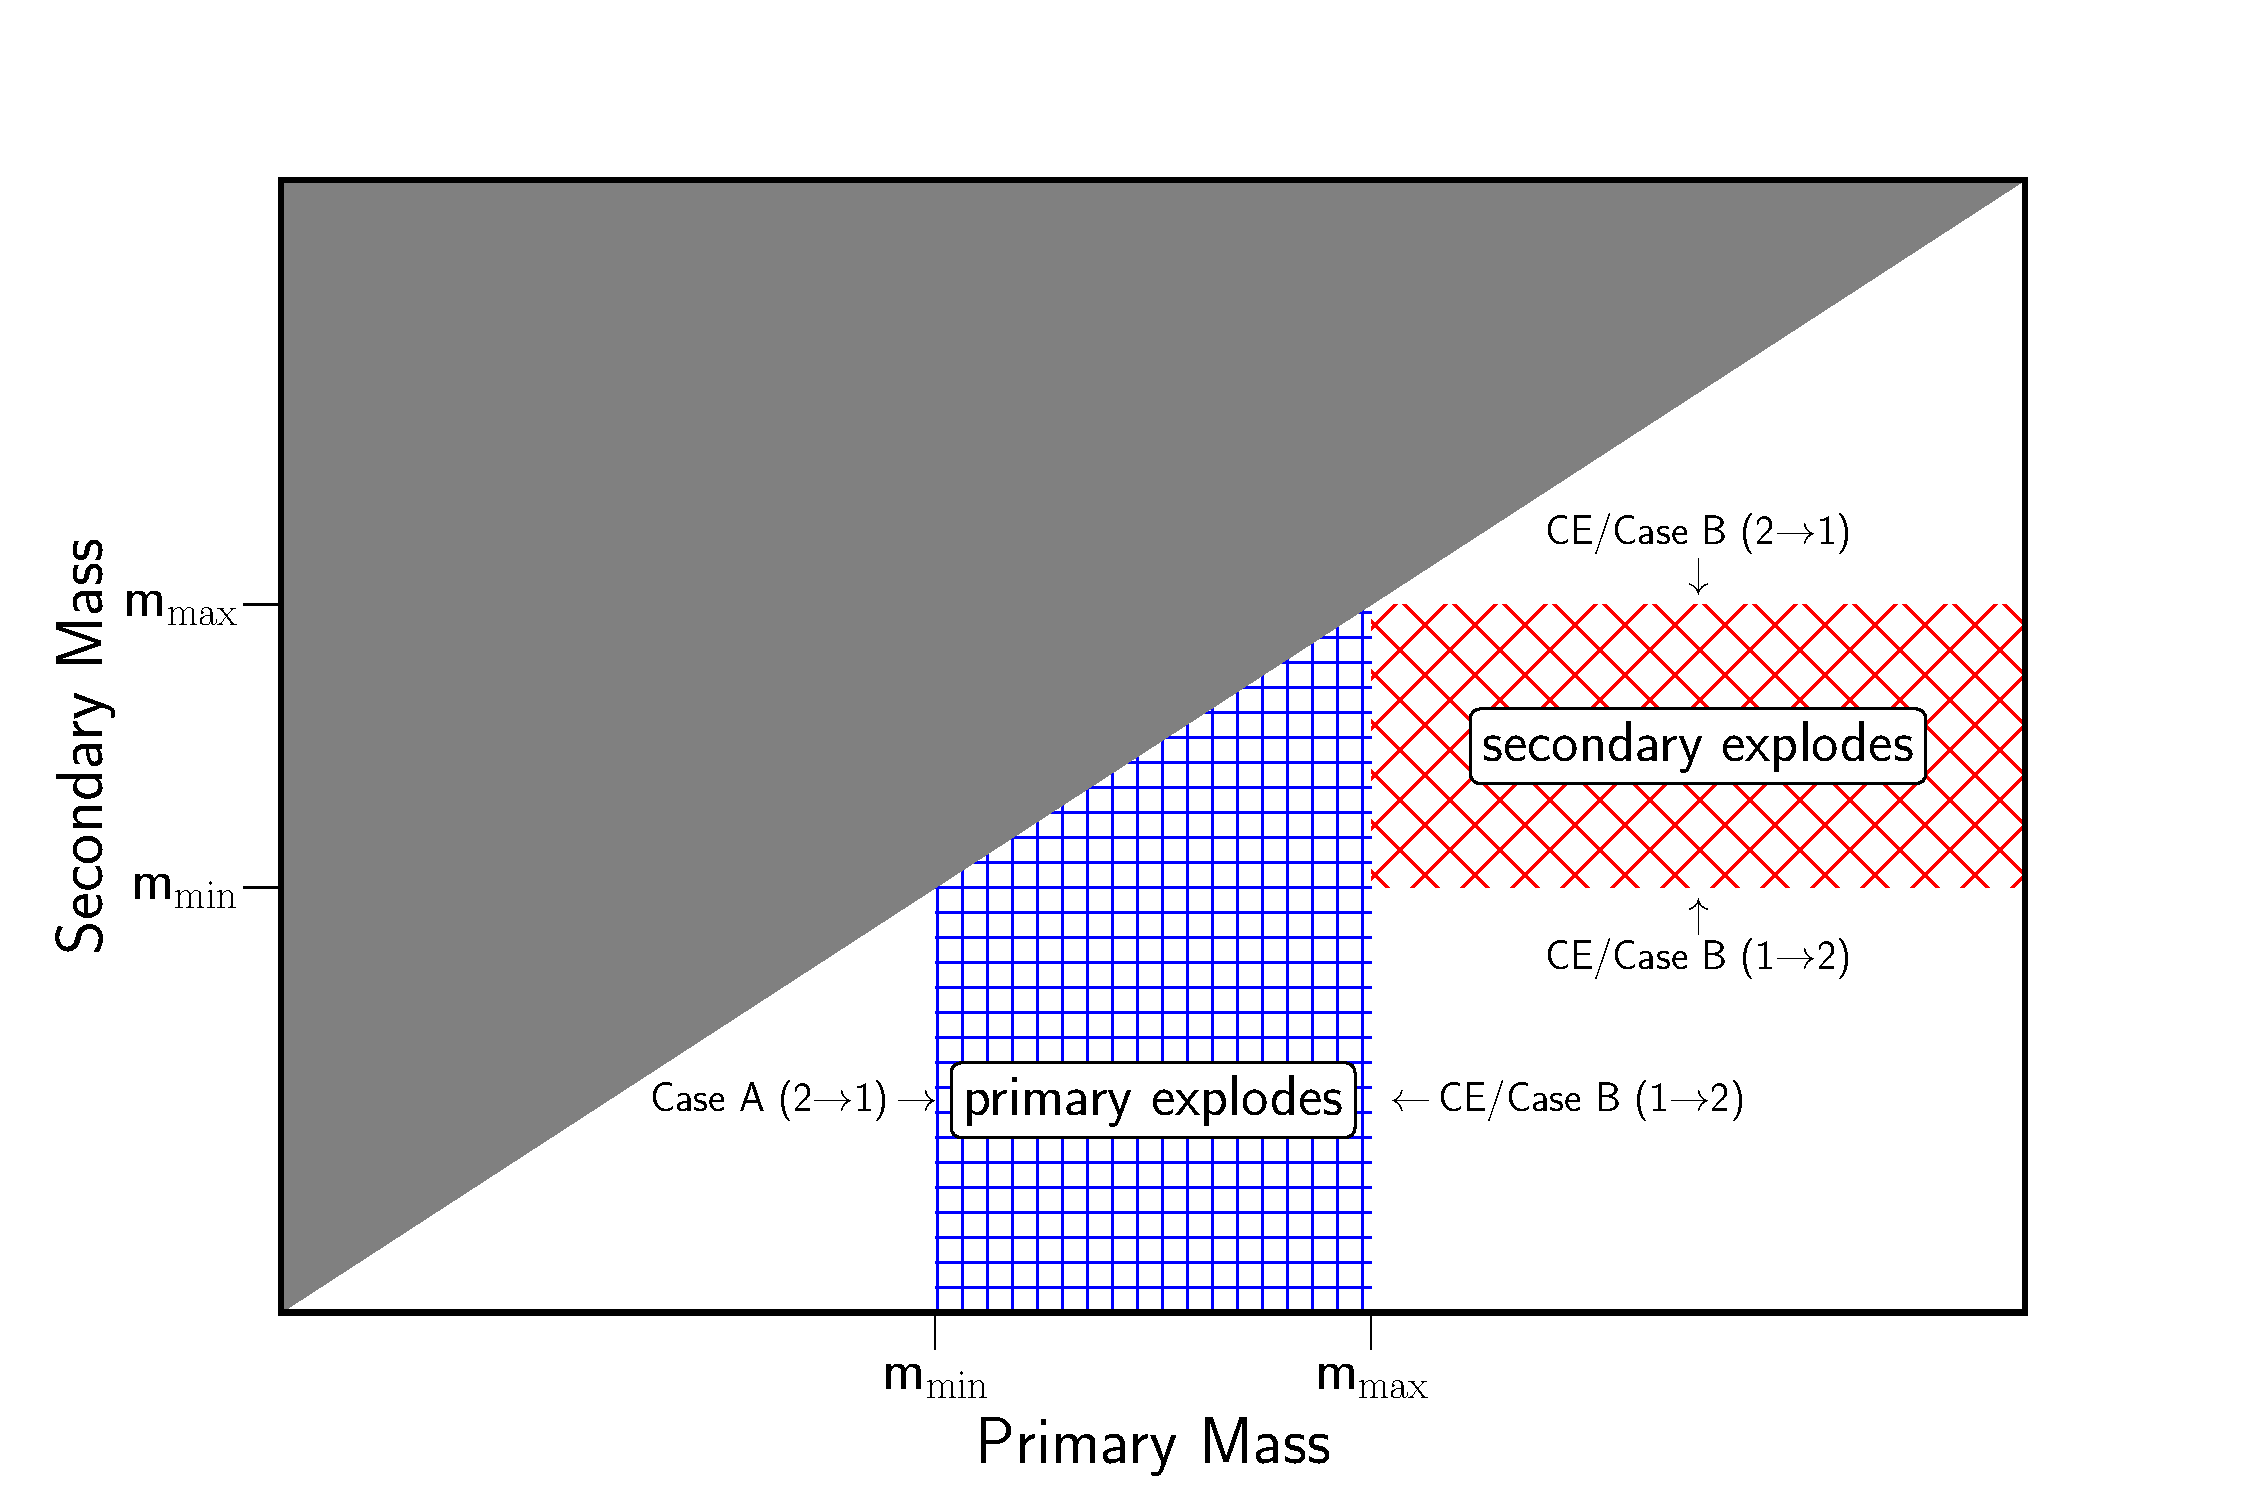
\includegraphics[width=1\textwidth]{../figures/chapter3/rates.pdf}
\caption{Overview of the different systems contributing to the \ia channel discussed here, on the mass-mass plane (see text).}
\label{fig:rates}
\end{center}
\end{figure*}

For binaries, the number of systems with ZAMS masses within a certain range (Figure\,\ref{fig:rates}) is:
\begin{equation}
n(m_1,m_2)dm_1dm_2 = m_1^{\alpha}q^{\kappa}dm_1dq,
\end{equation}
where $m_1$ is the mass of the primary, here defined as the initially more massive star, 
$q\equiv m_2/m_1\leq 1$ is the mass ratio, and $a,\kappa$ depend on the 
initial mass function (IMF) and mass-ratio distribution respectively. Integrating, one finds:
\begin{equation}\label{eq:3}
\begin{split}
N =  
\iint\limits_{m_{\rm min}\,q_{1}}^{m_{\rm max}\,q_{2}}m_1^{\alpha}q^{\kappa}dm_1dq  
 = f\frac{(m_{\rm min}^{\alpha+1} - m_{\rm max}^{\alpha+1})(q_{1}^{\kappa+1} -  q_{2}^{\kappa+1})}{(\alpha+1)(\kappa+1)}, 
\end{split}
\end{equation}
where $f$ is an appropriate normalization factor. 
Naively, one would expect the largest contribution from stars  that, in isolation, would be able to evolve
to the SAGB, viz. stars with ZAMS masses between $\sim 7$ and 11\msun\ \citep{Farmer:2015afs}. 
Since accretion is not required to trigger an explosion, 
\emph{all} primaries and secondaries inside this mass range 
can potentially contribute to $n_\star$. Hence, $(m_{\rm min},m_{\rm max})=(7,11)\msun;(q_1,q_2)=(0,1)$ for the primaries (blue region in 
Figure\,\ref{fig:rates}), and $(m_{\rm min},m_{\rm max})=(11,125)\msun;(q_1,q_2)=(7/11,1)$ for the secondaries (red region). For normalization, we consider all systems within $(m_{\rm min},m_{\rm max})=(0.1,125)\msun$. Adopting a 
\cite{Chabrier:2004vw} IMF with $a=-2.35$ for $m_1 \ge 1$, and a $q-$distribution with $k=-0.1$ \citep{Sana:2012px},
Eq.\,\ref{eq:3} yields, $n_{\rm \one}\times f_{\rm bin} \simeq 5.42\times 0.7=0.0039$ stars per \msun\ formed, with the largest contribution ($\sim 80\%$) expected from primaries. For $f_{\rm int}\simeq 1$, $n_\star$ would therefore exceed the number of \ia  integrated over a Hubble time, $n_{\rm \ia}\simeq0.002\msun^{-1}$ \citep{Maoz:2013hna}.

However, $f_{\rm int}$ is most likely smaller than unity. Firstly, only a fraction of 
the progenitor binary population will create naked helium stars. Most  systems within the 
hatched regions of Figure\,\ref{fig:rates} will transfer mass to their less massive 
companions after leaving the main sequence. For the majority of these cases, 
this  process will be  dynamically unstable, therefore leading to the removal of the envelope. If this process is indeed efficient, one would expect at least half of the stars to lose their envelopes, hence, conservatively, $f_{\rm int}\lesssim 0.5$ \citep{Sana:2012px}. 

Following the stripping of the envelope, any 
subsequent interaction should be sufficiently delayed, for the core to reach \mch. The post-CE orbital period distribution would generally favor slightly more compact configurations. Hence, only some fraction of the systems will be wide enough to allow 
 a second CE episode after the progenitor has expanded beyond $\sim 100\rsun$. 
Nonetheless, a fraction of the closer binaries that will undergo stable case BB Roche-lobe 
overflow (RLO), could still leave behind stripped \one cores of sufficiently high mass. For instance, the
 simulations of \cite{Tauris:2015xra} suggest that   a considerable number of helium-free \one proto-WDs 
with $m\simeq \mch$ can be produced via this channel. 

Considering some of the major uncertainties, conservatively, we expect: $0.1 \lesssim f_{\rm int}\lesssim 0.5$. 
Taking into account further ambiguities in the IMF and initial configurations, we conclude 
that $0.05\lesssim n_\star / n_{\rm \ia} \lesssim 1$. 
%\citep[see also][]{Jones:2018ule}.

Obviously, the above estimate omits most interactions that could move systems in and out of the hatched regions in 
Figure\,\ref{fig:rates}. Of particular importance may be interactions 
occurring before the helium-burning phase, as there are  
roughly three times as many systems with a total mass larger than 7\msun\  
than there are stars within the hatched regions of Figure\,\ref{fig:rates}. 
A fraction of this population can contribute significantly to the observed rate, after interacting via Case A/B RLO. 
Additional contributions may come from higher-order multiple systems and/or dynamical interactions in dense environments.  


Besides the integrated number of \ias, a property that is more challenging to match is the evolution of the \ia rate with cosmic time. \ias from this channel would have delay times dominated by the main sequence lifetime of the progenitors, i.e. of order 25 to 78\,Myr, for stars with ZAMS masses between 7 and 11\msun. Binaries interacting via early Case\,A RLO prior to the removal of the envelope, could contribute events up to $\sim 350$\,Myr following star formation. 

These delay times could help account for the high \ia rates in star-forming galaxies \citep{Maoz:2010pz,claeys2014}. 
However, some variant of the DD channel would still be required to explain events with much longer delay times.  

\section{Summary}\label{sec:5}
We have shown that stars able to form degenerate \one cores after losing 
their hydrogen  envelopes, are likely to explode as \ias instead of undergoing a core-collapse ECSN. 
For NeO compositions, the runaway seems to be triggered by the ignition of 
residual carbon following electron captures on \iso{Mg}{24}, which in turn 
leads to explosive oxygen burning at densities below $10^{9.77}$\,gr\,cm$^{-3}$ (Sections\,\ref{sec:2}). 
For hybrid CO/NeO cores, ignition is triggered by core compression, at a density of $10^{9.26}$\,gr\,cm$^{-3}$, similar to what is expected for CO WD deflagrations. For either case, the conditions at the onset of oxygen burning are such that the energetics  could resemble closely a typical \ias  (Section\,\ref{sec:3}). 
It would be worth considering whether the differences in density and 
composition could lead to distinct nucleosynthetic signatures that would help 
distinguish these progenitors and/or contribute uniquely to the chemical 
evolution of the Galaxy \citep[in analogy to ][for ECSNe]{Jones:2018ule}.



The frequency of the corresponding progenitor systems 
is sufficient to account for a considerable fraction of the observed \ia  rate  (Section\,\ref{sec:4}). Since, the bulk of events would occur only $\sim 50$\,Myr after star formation, this channel is mostly relevant to active late-type galaxies. The shorter delay times compared to traditional \ia scenarios, opens further interesting avenues for constraining this model, e.g. with low-metallicity stars.  

A similar \ia channel has  been proposed by \cite{waldman2006a} and \cite{waldman2008}, who have also demonstrated that some helium stars with \one cores can explode before any significant deleptonization occurs. However, these authors do not follow the final evolution stages, and their progenitors still retain a small He-rich envelope at the end. While here we demonstrate that the helium envelope is  likely lost only  after the core has grown to \mch, its evolution remains a major uncertainty for this progenitor channel. If helium is removed sufficiently early, e.g. due to binary interactions or dynamical instabilities, then this channel would instead create  sub-\mch\ \one\ WDs. 
%Goetz, Norbert, would you be able to add something here? 
In spite of the mass-loss uncertainties, if viable, this channel would help explain some of the observed \ia diversity. Since either star in binary system may potentially explode as a \ia without accreting from its  companion, the resulting events can resemble setups expected in both SD and DD scenarios. Explosions resulting from the explosion of the secondary, would follow a first core-collapse SN. This could lead to \ia remnants with no luminous surviving stars, high proper motions due to a kick from the first SN \cite[like the Kepler remnant,][]{Chiotellis:2011jy}, and possibly associated with a neutron star. 
Since the  envelope can be removed either due to winds, case-BB mass transfer, or a common envelope event, some diversity is also expected in the SN environment. In turn this would influence bot the appearance of the explosion and the evolution of the SN remnant. 

Finally this channel seems relevant to other emerging correlations, e.g. the one found between SN locations and the velocity of Si features, or the apparent correlation between \ia rate and IMF variations at low masses \citep{Maoz:2013hna}.
	
\newpage  % Inserting empty page
\mbox{}
\thispagestyle{empty}
	

	
\end{document}